\chapter{Human--computer interaction}
\label{ch:Human-computer interaction}
Human--computer interaction is a multi-disciplinary research area that covers user interface design, hardware, software, social aspects, and more. Important concepts in this research area are usability and user experience.

With new technologies such as novel input devices and increased computational power come new possibilities. The present work makes use of these possibilities, using novel user input devices for structural modeling and increased computational power for real-time structural analysis. 

\section{Direct manipulation}
Direct manipulation is a human--computer interaction style characterized by the continuous representation of objects of interest with rapid, reversible, and incremental feedback \cite{Shneiderman1982}. Users can directly manipulate objects on the screen using real-world metaphors, which engages the users with their task and encourages further explorations \cite{Shneiderman:1997:DMC:238218.238281}. This is achieved by reducing the perceptual and cognitive resources required to understand and use the interface \cite{Sears1990}.

\section{Visualizations}
Scientific visualization is a subfield of computer graphics. The purpose of scientific visualization is to graphically illustrate scientific data. This is also important in conceptual structural design software, as visualizing the design result is of great importance. The visualization should be such that the user can quickly interpret the result and gain insight from it. 

\begin{figure}
  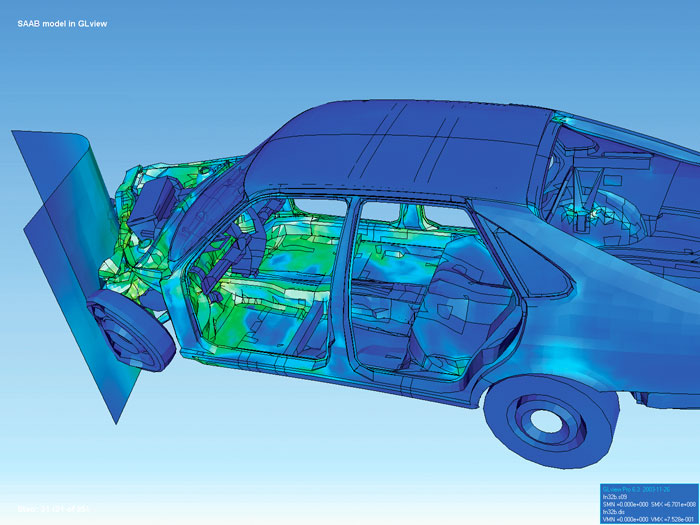
\includegraphics[width=320pt]{graphics/car.jpg}
  \caption{Visualization of how a car deforms in an asymmetrical crash using finite element analysis.}
  \label{fig:Car}
\end{figure}

Figure \ref{fig:Car} shows an example of how the results of computational analysis can be visualized. The original geometry of an undeformed car is modified with the computed displacements. The geometry, in this case the car, is also colored according to some selected condition, e.g., von Mises tension, shear force, bending moment. 

Edward Tufte is a pioneer in the field of data visualization \cite{tufte1997visual, tufte1990envisioning, tufte2001the}. His principles of graphical excellence can be stated as follows \cite{tufte2001the}:

\begin{itemize} 
\item Graphical excellence is the well-designed presentation of interesting data--–a matter of substance, of statistics and design.
\item Graphical excellence consists of complex ideas communicated with clarity, precision and efficiency.
\item Graphical excellence is that which gives to the viewer the greatest number of ideas in the shortest time with the least ink in the smallest space.
\end{itemize} 

\section{Technology}
The introduction of input devices such as the mouse and joystick significantly improved human--computer interaction with interfaces that adapted accordingly \cite{Sears1990}. When the touch screen was introduced, it had a vital advantage over all these devices---the user could literally touch objects on the screen to manipulate them, creating a very direct method of inputting information \cite{Sears1990}. This closed the gap between the human and the computer.

There is a wide variety of interaction techniques that create direct manipulation interfaces for three-dimensional (3D) applications using two-dimensional (2D) input devices such as the mouse \cite{Nielson:1987:DMT:319120.319134}. However, as such input devices have one degree of freedom less than the 3D user interface, there will always exist a need for some form of gestures. 

The Leap Motion Controller \cite{LeapMotion2013} is a relatively small and simple input device that is placed in front of the keyboard. The controller then tracks the user’s hands across the controller’s field of vision. Combined with a software development kit (SDK), the controller creates a computational model of the user’s hands, which can then be used to interact with software in three dimensions. This enables very direct manipulations for 3D user interfaces.

Computer games have led the development of novel input devices along with new styles of games to address some limitations of conventional systems \cite{Kosmadoudi2013}, e.g., the Wii remote \cite{Nintendo}, Microsoft’s Kinect for Xbox \cite{Microsoft}, and the PlayStation Move \cite{Playstationa}. These novel input devices have moved away from the conventional human--computer interaction to invoke an intuitive interface that supports the natural human approach to interaction. For a long time, games have been perceived as fun and engaging, and many different research disciplines have investigated whether gaming methods can be used to improve human--computer interactions to create more effective, immersive, and engaging forms of learning or training \cite{Kosmadoudi2013}. 

Interest in the development of virtual reality glasses has recently increased as products such as the Oculus Rift \cite{Oculus} and PlayStation’s Project Morpheus \cite{Playstation} have become widely available. These virtual reality glasses have primarily been developed for games, but have received interest from other fields, e.g., to help students understand complex structural behavior \cite{fogarty2014exploring}.

